\chapter{Ergebnisse}


- Auswertung (Qualitative Auswertung)\\
- Lauferkennung \\
- Rechenzeit: kein wesentlicher Unterschied (55 Sec und 57 Sec)


\section{Lauferkennung}

\begin{figure}[H]
	\centering
	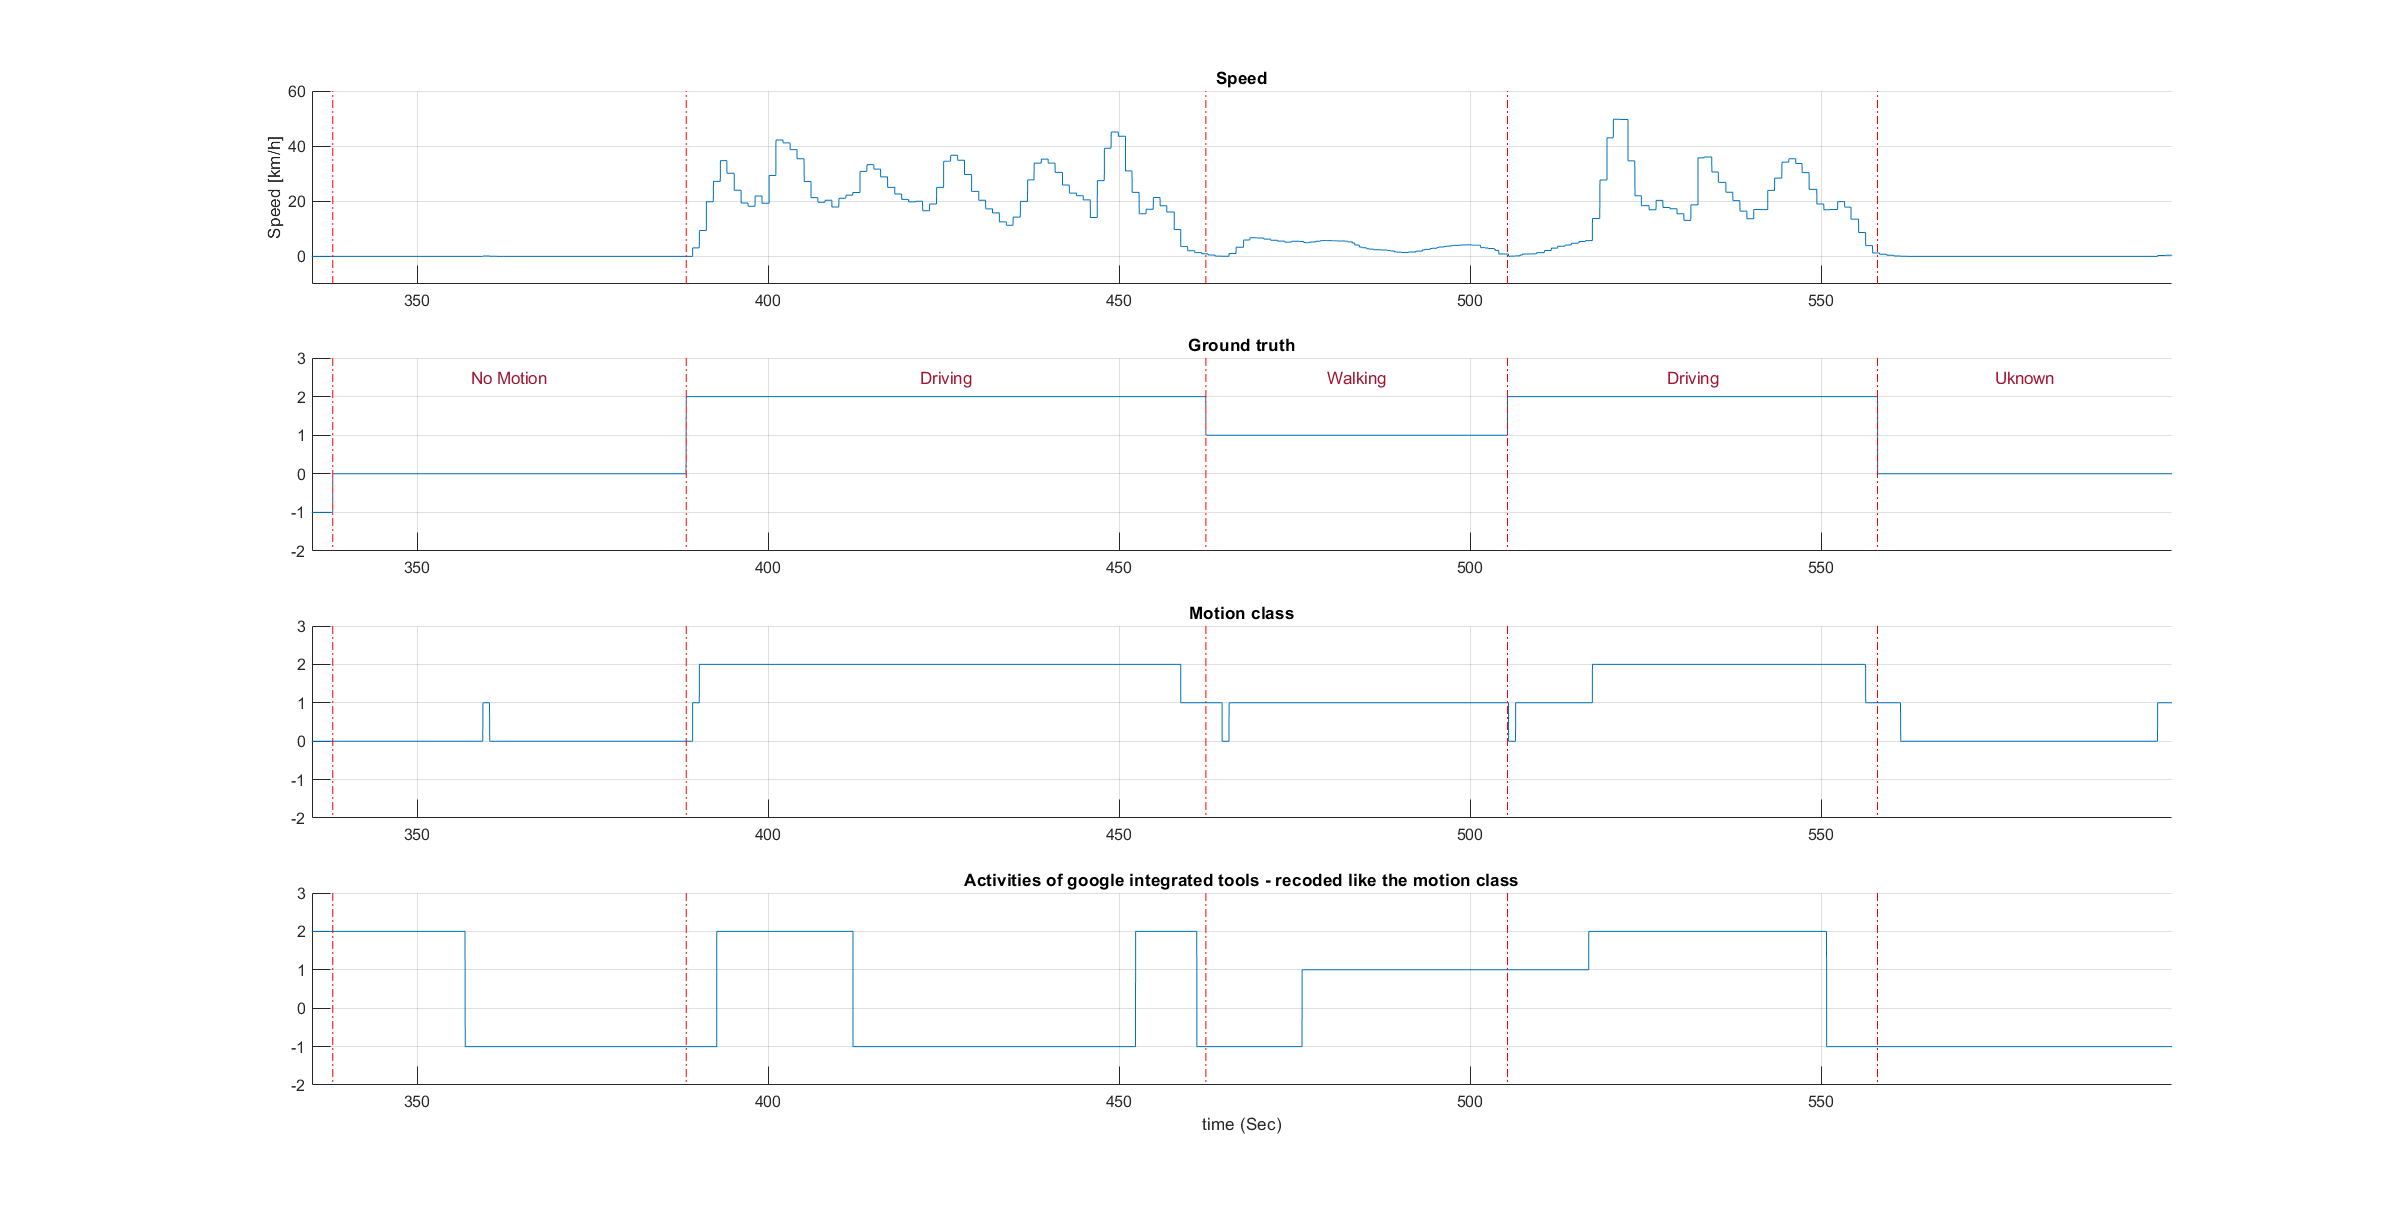
\includegraphics[width=\linewidth]{Bilder/Speed_Groundtruth_MotionClass_GoogleMD_Compare.png}
	\caption{Ergebnis des Lauferkkennungsmodells}
	\label{fig:Speed_Groundtruth_MotionClass_GoogleMD_Compare}
\end{figure}



\section{Verschiedene Fahrerpositionierung}

\begin{figure}[H]
	\centering
	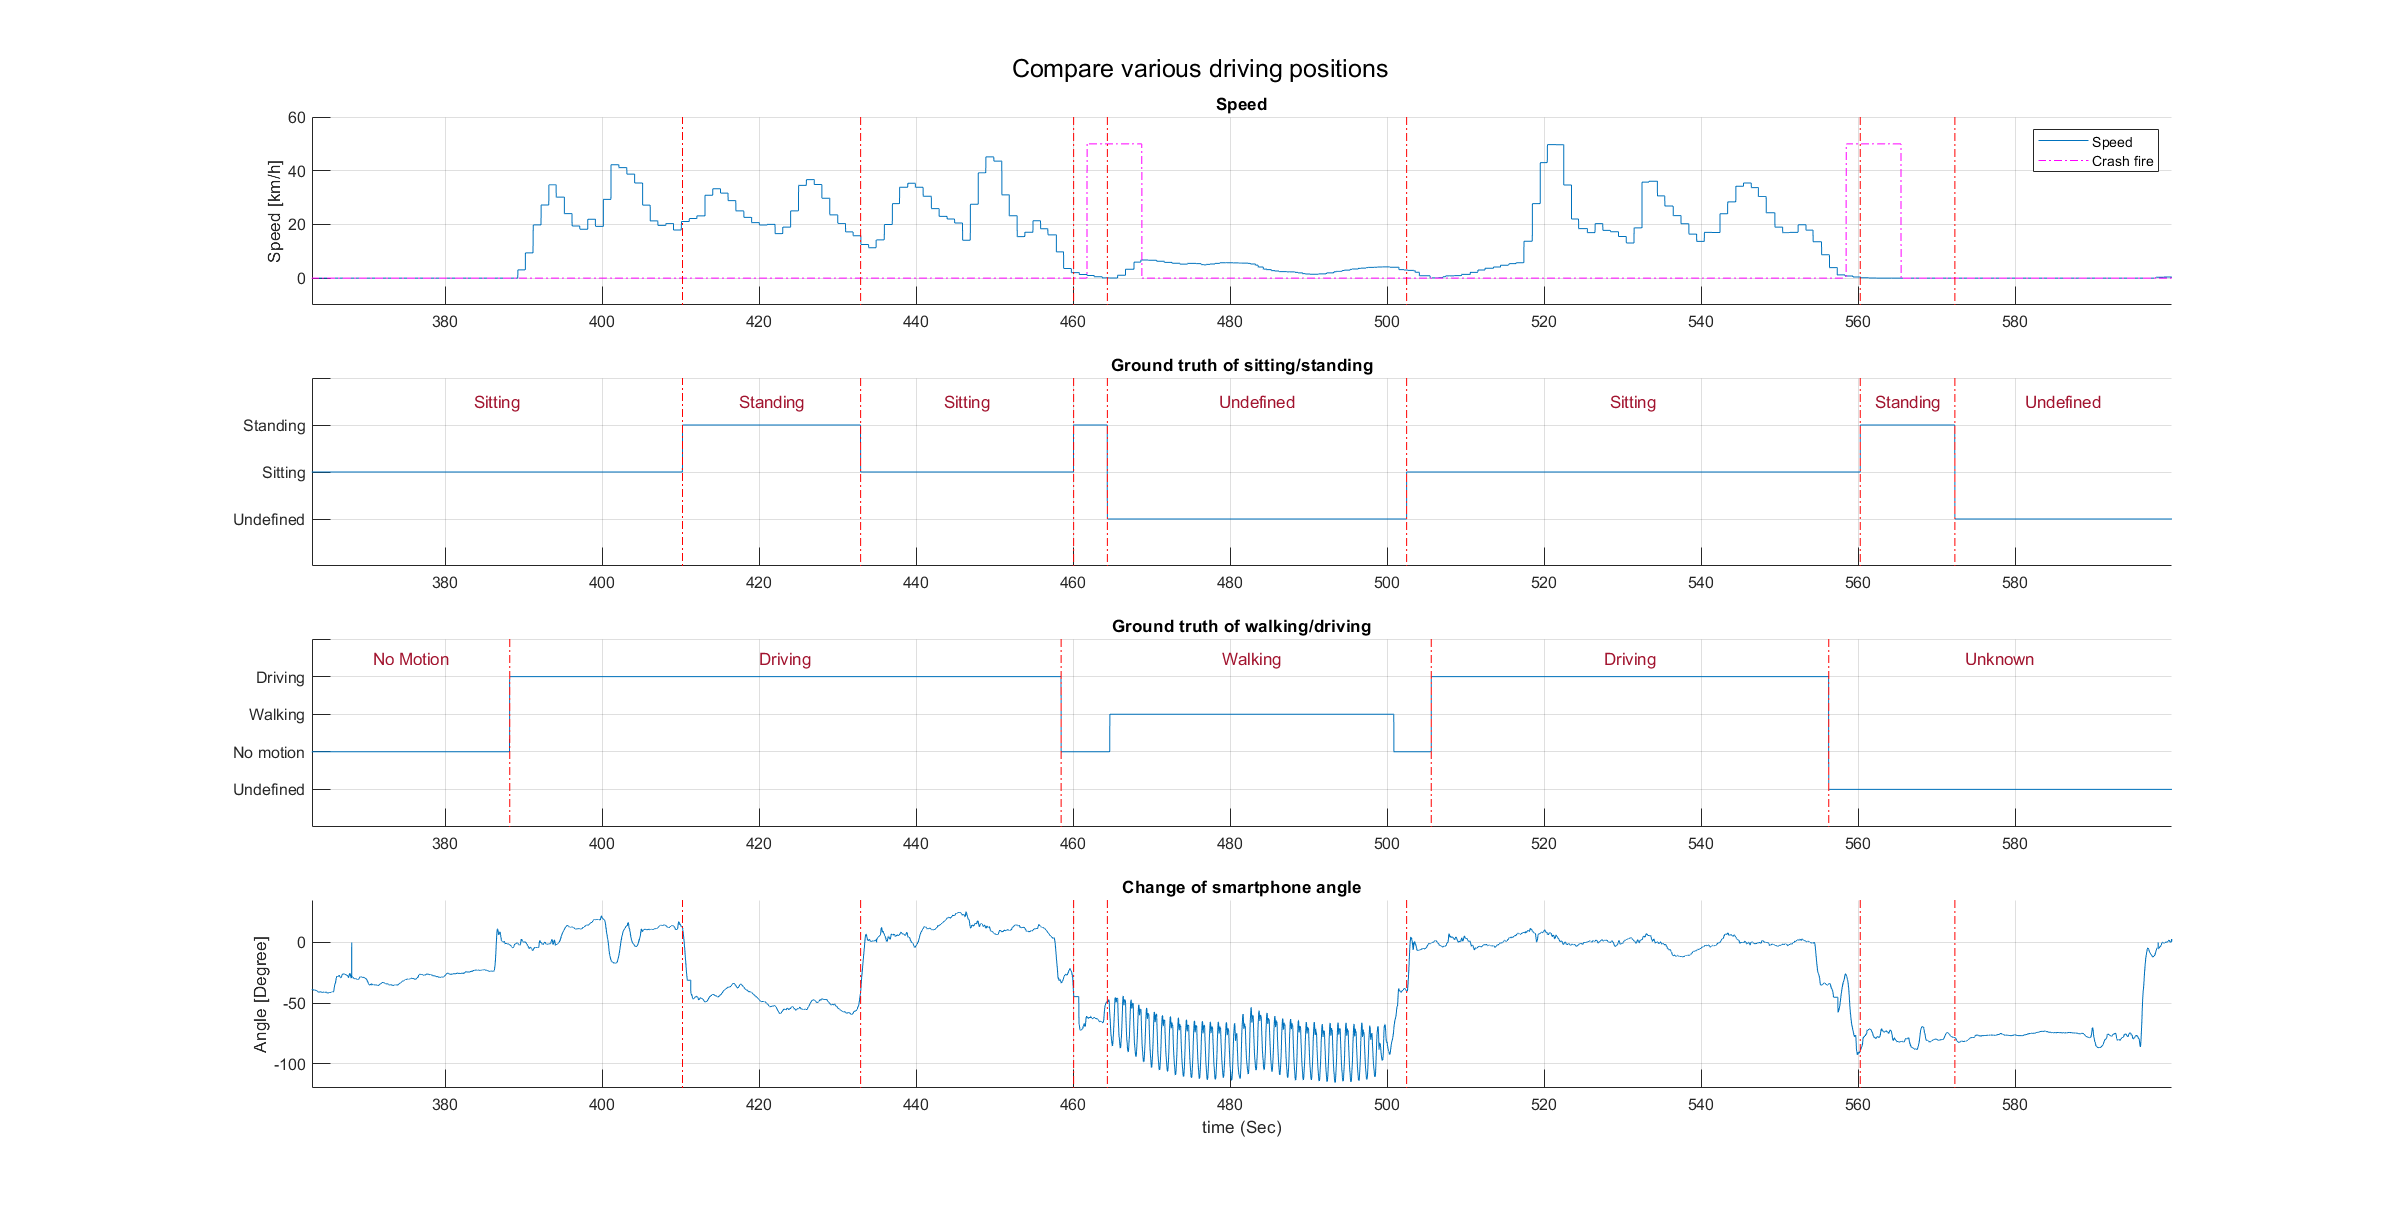
\includegraphics[width=\linewidth]{Bilder/Speed_Groundtruth_WalkStand_Compare.png}
	\caption{Vergleich der Fahrt in vertikaler und normaler Position}
	\label{fig:Speed_Groundtruth_WalkStand_Compare}
\end{figure}

\section{Anhalten}

\begin{figure}[H]
	\centering
	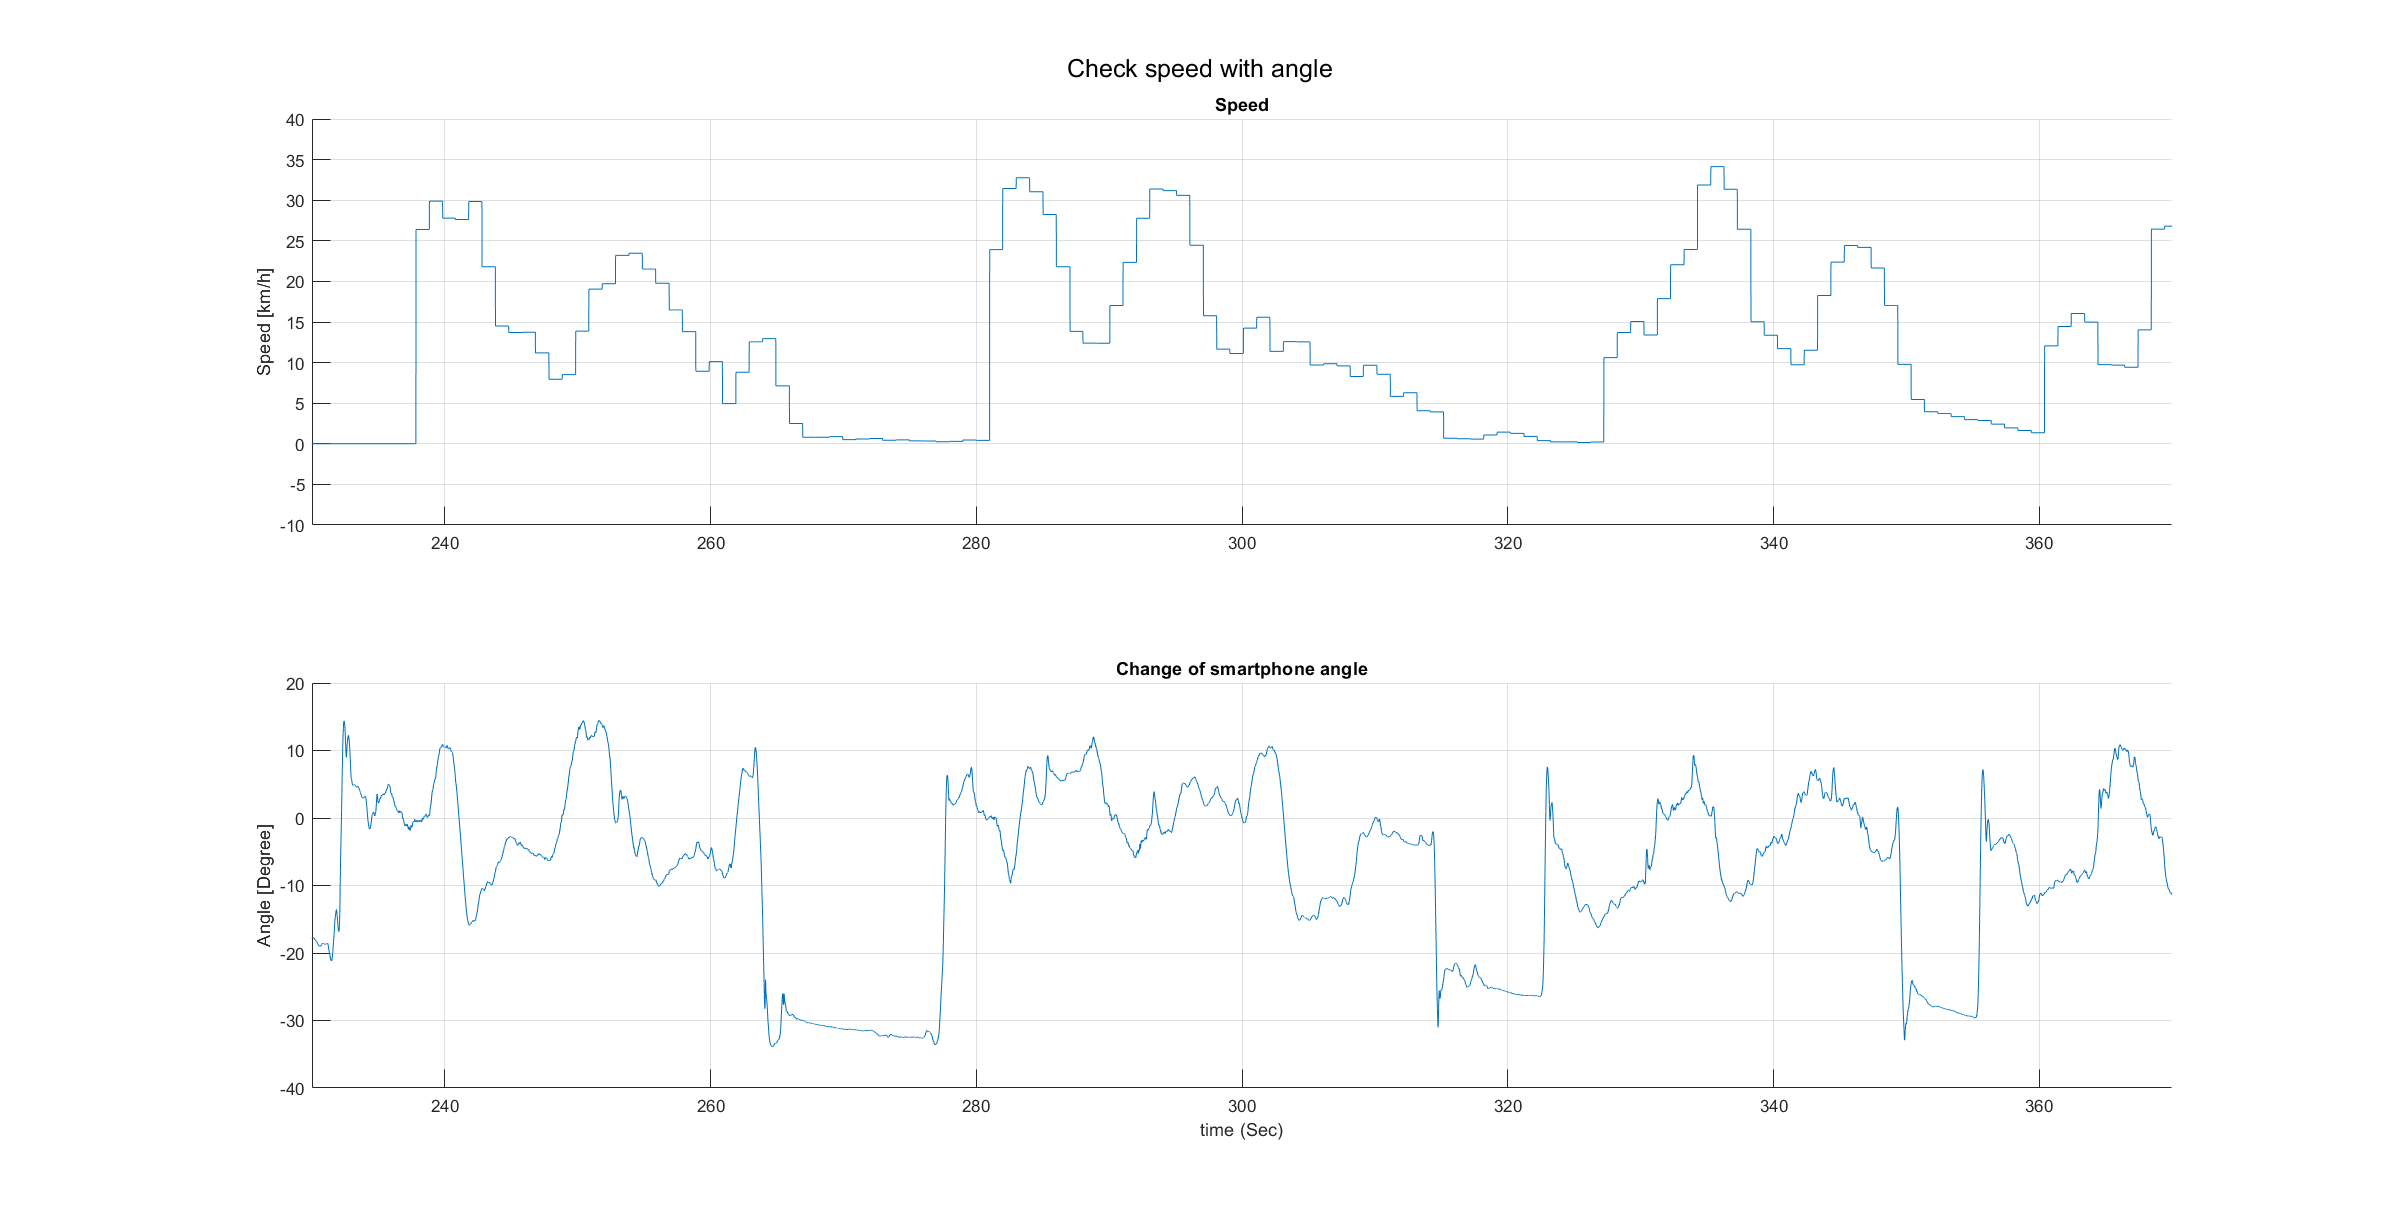
\includegraphics[width=\linewidth]{Bilder/Speed_AngleChangeCompare.png}
	\caption{Winkeländerung des Smartphones durch das Anhalten}
	\label{fig:Speed_AngleChangeCompare}
\end{figure}
Winkeländerung nicht über \ang{45} beträgt $->$ kein Fehlalarm.\\
\\
Beurteilung:

Zu diesem Zweck wurde einen einfachen Test durchgeführt. Der Test hat keine falsche Alarmauslösungen aktiviert. Grund ist, dass die Winkeländerung nicht \ang{90} beträgt sondern nur ca. \ang{20}-\ang{30} (\autoref{fig:MotorbikeDrivingStanding}). Die Person hat sein Bein beim Sitzen nicht genau horizontal sondern leicht nach Unten geneigt. Und wenn der Fahrer sein Fuß runter setzt, ist diese auch nicht genau vertikal sondern bisschen gebogen mit einem Winkel von ca. \ang{10}-\ang{20} zum Vertikallinie. D.h. die Winkeländerung nicht \ang{90} ist.

\begin{figure}[H]
	\centering
	\begin{subfigure}{\textwidth}
		\centering
		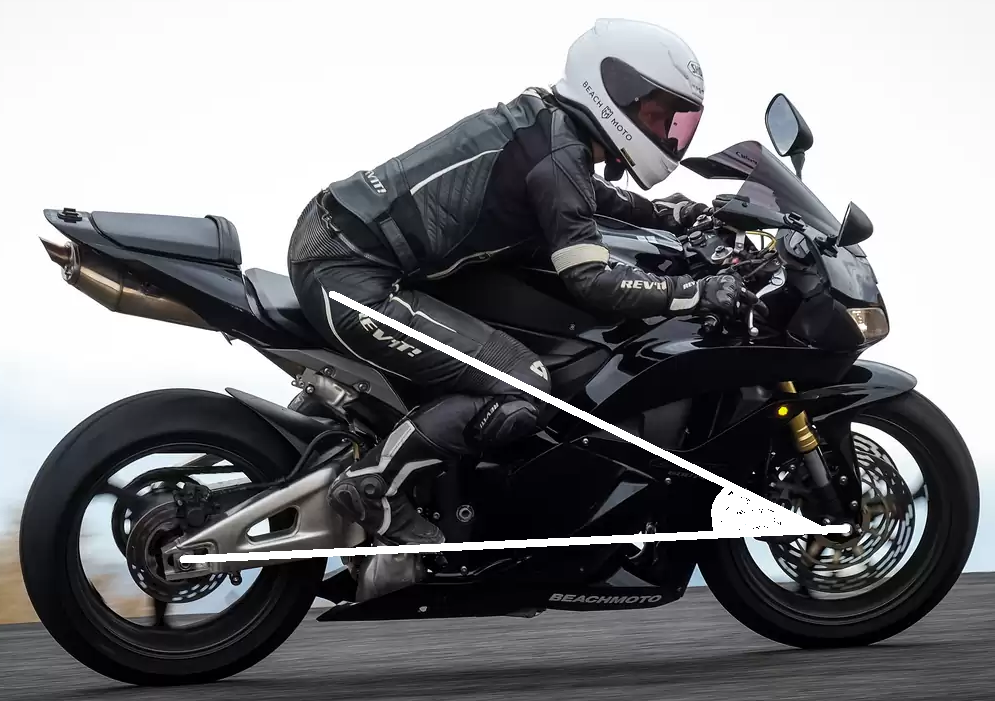
\includegraphics[width=0.5\textwidth]{Bilder/MotorbikeDriving2.png}
		\caption{Beinposition während einer Fahrt}
		\label{fig:MotorbikeDriving}
	\end{subfigure}
	\hfill
	\begin{subfigure}{\textwidth}
		\centering
		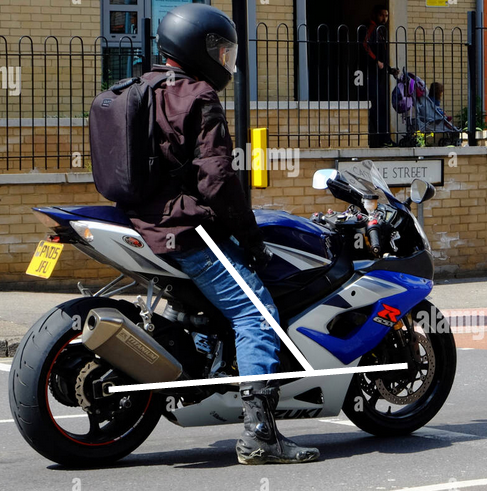
\includegraphics[width=0.5\textwidth]{Bilder/MotorbikeStanding2.png}
		\caption{Beinposition Beim Stehen}
		\label{fig:MotorbikeStanding2}
	\end{subfigure}
	\caption{Beinpositionen während einer Fahrt und gestreckt}
	\label{fig:MotorbikeDrivingStanding}
\end{figure}



\section{Verifikationsversuche}

- Alle geplanten Szenarien wurden mind. einmal getestet.\\

- Die erste sowie letzte Szenarien wurden jeweils zweimal getestet.\\


\section{Vor- und Nachteile}
- Rechenzeit: kein wesentlicher Unterschied (55 Sec und 57 Sec)





 